\documentclass[10pt]{beamer}

\usetheme[progressbar=frametitle]{metropolis}
\usepackage{appendixnumberbeamer}
\usepackage[compat=1.0.0]{tikz-feynman}

\title{Building SUSY models II: using superfields}
\subtitle{Seminar on Supersymmetry and its breaking}
\author{Matteo Zortea}
\date{Universit\"at Heidelberg, $27^{th}$ May 2022}
\institute{Coordinated by prof. J\"org J\"ackel}

\makeatletter
\setbeamertemplate{title page}{
  \begin{minipage}[b][\paperheight]{\textwidth}
    \centering  % <-- Center here
    \ifx\inserttitlegraphic\@empty\else\usebeamertemplate*{title graphic}\fi
    \vfill%
    \ifx\inserttitle\@empty\else\usebeamertemplate*{title}\fi
    \ifx\insertsubtitle\@empty\else\usebeamertemplate*{subtitle}\fi
    \usebeamertemplate*{title separator}
    \ifx\beamer@shortauthor\@empty\else\usebeamertemplate*{author}\fi
    \ifx\insertdate\@empty\else\usebeamertemplate*{date}\fi
    \ifx\insertinstitute\@empty\else\usebeamertemplate*{institute}\fi
    \vfill
    \vspace*{1mm}
  \end{minipage}
}

\setbeamertemplate{title}{
%  \raggedright%  % <-- Comment here
  \linespread{1.0}%
  \inserttitle%
  \par%
  \vspace*{0.5em}
}
\setbeamertemplate{subtitle}{
%  \raggedright%  % <-- Comment here
  \insertsubtitle%
  \par%
  \vspace*{0.5em}
}
\makeatother




\begin{document}
\begin{frame}
\titlepage
\end{frame}

\begin{frame}{Main points of the talk}
\begin{itemize}
    \item Apply the superspace formalism and show why it is useful to build SUSY theories
    \item Principles to construct SUSY lagrangians 
    \item SUSY gauge theories: QED and QCD
    \item SUSY predictions: particles, interaction, masses, ...
    \item N=1 nonrenormalization theorem
\end{itemize}
\end{frame}

\begin{frame}{How to build SUSY invariant lagrangians}
    We want our theory to be SUSY invariant, that is
    \begin{equation*}
        \left(\epsilon \hat Q + \epsilon^\dagger \hat Q\right) S = \left(\epsilon \hat Q + \epsilon^\dagger \hat Q\right) \int dx^\mu \mathcal{L} = 0
    \end{equation*}
    We know that this condition is met if, under a given transformation
    \begin{equation*}
        \mathcal{L} \to \mathcal{L} + \partial_\mu f
    \end{equation*}
    Hence our goal is to build a lagrangin which transforms in this way, using \textbf{Chiral} ($\bar D_{\dot\alpha} \Phi = 0$ or $D_{\alpha}\Phi^* = 0$) and \textbf{Vector} ($V=V^*$) superfields
\begin{gather*}
    \Phi(x, \theta, \bar\theta) = \phi(x) + i\bar\theta \bar\sigma^{\mu}\theta \partial_{\mu}\phi(x) + \frac{1}{4}\theta\theta\bar\theta\bar\theta\partial_{\mu}\partial^{\mu}\phi(x) + \sqrt{2}\theta\psi(x) + \\ 
    -\frac{i}{\sqrt{2}}\theta\theta\bar\theta\bar\sigma^{\mu}\partial_{\mu}\psi(x) + \theta\theta \underbrace{F(x)}_{\text{F term}} \\
    V\left(x, \theta, \bar\theta\right) = a+\theta \xi+\bar\theta \xi^* +\theta \theta b+\bar\theta \bar\theta b^{*}+\bar\theta \bar{\sigma}^{\mu} \theta A_{\mu}+ \\ 
    + \bar\theta \bar\theta \theta\left(\lambda-\frac{i}{2} \sigma^{\mu} \partial_{\mu} \xi^*\right)
    +\theta \theta \bar\theta\left(\lambda^*-\frac{i}{2} \sigma^{\mu} \partial_{\mu} \xi\right)+\theta \theta \bar\theta \bar\theta \underbrace{\left(\frac{1}{2} D+\frac{1}{4} \partial_{\mu} \partial^{\mu} a\right)}_{\text{D term}}
\end{gather*}
\end{frame}

\begin{frame}{How to build SUSY invariant lagrangians}
General superfield expansion
\begin{equation*}
    S\left(x, \theta, \bar\theta\right)=a+\theta \xi+\bar\theta \chi^{\dagger}+\theta \theta b+\bar\theta \bar\theta c+\bar\theta \bar{\sigma}^{\mu} \theta v_{\mu}+\bar\theta \bar\theta \theta \eta+\theta \theta \bar\theta \zeta^{\dagger}+\theta \theta \bar\theta \bar\theta d
\end{equation*}
For the chiral field $\Phi(x, \theta \bar\theta)$ components one has the following transformation properties
\begin{gather*}
    \delta\phi = \sqrt{2} \zeta \psi \\
    \delta\psi_\alpha = -\sqrt{2}F\zeta_{\alpha} - i \sqrt{2} \sigma^{\mu}_{\alpha \dot\alpha} \bar\zeta^{\dot \alpha} \partial_\mu \phi \\
    \boxed{\delta_{\epsilon} F = -i\epsilon^{\dagger} \bar\sigma^\mu \partial_\mu \psi}
\end{gather*}
For the vector field $V(x, \theta, \bar\theta)$ components one has
\begin{gather*}
        \sqrt{2} \delta_{\epsilon} a =\epsilon \xi+\epsilon^{\dagger} \xi^{\dagger} \qquad 
        \sqrt{2} \delta_{\epsilon} \xi_{\alpha} =2 \epsilon_{\alpha} b-\left(\sigma^{\mu} \epsilon^{\dagger}\right)_{\alpha}\left(A_{\mu}+i \partial_{\mu} a\right) \\
        \sqrt{2} \delta_{\epsilon} b =\epsilon^{\dagger} \lambda^{\dagger}-i \epsilon^{\dagger} \sigma^{\mu} \partial_{\mu} \xi \qquad
        \sqrt{2} \delta_{\epsilon} A^{\mu} =i \epsilon \partial^{\mu} \xi-i \epsilon^{\dagger} \partial^{\mu} \xi^{\dagger}+\epsilon \sigma^{\mu} \lambda^{\dagger}-\epsilon^{\dagger} \bar{\sigma}^{\mu} \lambda \\
        \sqrt{2} \delta_{\epsilon} \lambda_{\alpha} =\epsilon_{a} D+\frac{i}{2}\left(\sigma^{\mu} \sigma^{\nu} \epsilon\right)_{\alpha}\left(\partial_{\mu} A_{\nu}-\partial_{\nu} A_{\mu}\right) \\
        \boxed{\sqrt{2} \delta_{\epsilon} D =-i \epsilon \sigma^{\mu} \partial_{\mu} \lambda^{\dagger}-i \epsilon^{\dagger} \bar{\sigma}^{\mu} \partial_{\mu} \lambda}
\end{gather*}
\end{frame}

\begin{frame}{How to build SUSY invariant lagrangians}
Idea $\rightarrow$ "select" the components of the fields that transforms as total derivatives
\begin{equation*} 
    \mathcal{L}[\Phi, V] = \alpha \, \left[V\right]_D + \beta \, \left[\Phi\right]_F  + \gamma \, \left[\Phi^*\right]_F
\end{equation*}
How can we "pick" only the terms we need? $\rightarrow$ Grassman integration
\begin{gather*}
    \int d^2\theta \ \theta^\alpha \, f(x, \bar\theta) = f(x, \bar\theta) \, \delta_{\alpha, 2} \\
    \int d^2\theta d^2\bar\theta  \ \bar\theta^\alpha \theta^\beta f(x) = f(x) \, \delta_{\alpha, 2} \, \delta_{\beta, 2}
\end{gather*}
Hence we are interested in
\begin{gather*}
    \left[\Phi\right]_F = \int d^2\theta \Phi + \text{total derivative} \\
    \left[V\right]_D = \int d^2\theta d^2\bar\theta V(x, \theta, \bar\theta) + \text{total derivative}
\end{gather*}
\end{frame}

\begin{frame}{How to build SUSY invariant lagrangians}
    Let us focus for a moment on the D term.\\
    A vector field can be obtained from 2 chiral superfields by taking the product $\Phi^*\Phi$
    \begin{gather*}
        \Phi(x, \theta, \bar\theta) = \phi(x) + i\bar\theta \bar\sigma^{\mu}\theta \partial_{\mu}\phi(x) + \frac{1}{4}\theta\theta\bar\theta\bar\theta\partial_{\mu}\partial^{\mu}\phi(x) + \sqrt{2}\theta\psi(x)\\ 
        -\frac{i}{\sqrt{2}}\theta\theta\bar\theta\bar\sigma^{\mu}\partial_{\mu}\psi(x) + \theta\theta F(x) \\
            \Phi^{* i} \Phi_{j}= \phi^{* i} \phi_{j}+\sqrt{2} \theta \psi_{j} \phi^{* i}+\sqrt{2} \theta^{\dagger} \psi^{\dagger i} \phi_{j}+\theta \theta \phi^{* i} F_{j}+\theta^{\dagger} \theta^{\dagger} \phi_{j} F^{* i} \\
            +\theta^{\dagger} \bar{\sigma}^{\mu} \theta\left[i \phi^{* i} \partial_{\mu} \phi_{j}-i \phi_{j} \partial_{\mu} \phi^{* i}-\psi^{\dagger i} \sigma_{\mu} \psi_{j}\right] \\
                +\frac{i}{\sqrt{2}} \theta \theta \theta^{\dagger} \bar{\sigma}^{\mu}\left(\psi_{j} \partial_{\mu} \phi^{* i}-\partial_{\mu} \psi_{j} \phi^{* i}\right)+\sqrt{2} \theta \theta \theta^{\dagger} \psi^{\dagger i} F_{j} \\
                +\frac{i}{\sqrt{2}} \theta^{\dagger} \theta^{\dagger} \theta \sigma^{\mu}\left(\psi^{\dagger i} \partial_{\mu} \phi_{j}-\partial_{\mu} \psi^{\dagger i} \phi_{j}\right)+\sqrt{2} \theta^{\dagger} \theta^{\dagger} \theta \psi_{j} F^{* i} \\
                +\theta \theta \theta^{\dagger} \theta^{\dagger}\left[F^{* i} F_{j}-\frac{1}{2} \partial^{\mu} \phi^{* i} \partial_{\mu} \phi_{j}+\frac{1}{4} \phi^{* i} \partial^{\mu} \partial_{\mu} \phi_{j}+\frac{1}{4} \phi_{j} \partial^{\mu} \partial_{\mu} \phi^{* i}\right. \\
                \left.+\frac{i}{2} \psi^{\dagger i} \bar{\sigma}^{\mu} \partial_{\mu} \psi_{j}+\frac{i}{2} \psi_{j} \sigma^{\mu} \partial_{\mu} \psi^{\dagger i}\right]
    \end{gather*}
\end{frame}
\begin{frame}{How to build SUSY invariant lagrangians}
    Now "select" the SUSY invariant component (D component)
    \begin{gather*}
        \left[\Phi^*\Phi\right]_D = \int d^2\theta d^2\bar\theta \ \Phi^*(x, \theta, \bar\theta) \Phi(x, \theta, \bar\theta) \\
        \left[F^* F - \frac{1}{2} \partial^{\mu} \phi^{* i} \partial_{\mu} \phi_{j}+\frac{1}{4} \phi^{* i} \partial^{\mu} \partial_{\mu} \phi_{j}+\frac{1}{4} \phi_{j} \partial^{\mu} \partial_{\mu} \phi^{* i}\right. \\
                \left.+\frac{i}{2} \psi^{\dagger i} \bar{\sigma}^{\mu} \partial_{\mu} \psi_{j}+\frac{i}{2} \psi_{j} \sigma^{\mu} \partial_{\mu} \psi^{\dagger i}\right] = \\
        = -\partial^{\mu}\phi^*\partial_{\mu}\phi + i\psi^{\dagger}\bar\sigma^{\mu}\partial_{\mu}\psi + F^*F + \text{total derivative}
    \end{gather*}
    Hence 
    \begin{equation*}
        \boxed{S = \int dx^{\mu} \mathcal{L} = \int dx^{\mu} -\partial^{\mu}\phi^*\partial_{\mu}\phi + i\psi^{\dagger}\bar\sigma^{\mu}\partial_{\mu}\psi + F^*F}
    \end{equation*}
    \centerline{\bfseries $\rightarrow$ Free Wess-Zumino model!}
\end{frame}

\begin{frame}{How to build SUSY invariant lagrangians}
    In order to add SUSY invariant interactions, let us recall the definitions of chiral superfields 
    \begin{equation*}
        \bar D_{\dot\alpha} \Phi = 0 \qquad D_{\alpha} \Phi^* = 0
    \end{equation*}
        Noote that any analytic function of chiral superfields is in turn a chiral superfield (power series expansion and product rule). \\
        $\Rightarrow$ Write our chiral term of $N$ fields as 
        \begin{equation*}
            W(\{\Phi_k\}) = \sum_i^N a_i \Phi_i + \sum_{i,j}^N \frac{1}{2!} m_{ij} \Phi_{i}\Phi_j + \sum_{i,j,k}^N \frac{1}{3!} y_{ijk} \Phi_i \Phi_j \Phi_k
        \end{equation*}
        Higher order terms are non-renormalisable. \\
        Reality of the action requires us to take $W + W^*$
    
\end{frame}

\begin{frame}{How to buld SUSY invariant lagrangians}
\begin{gather*}
\mathcal{L}_{WZ}\left(\{\Phi_i\}, \{\Phi^*_i\}\right) = \mathcal{L}_{WZ,D} + \mathcal{L}_{WZ,F} = \\
= \left[\Phi^{*i}\Phi^i\right]_D + \left[W(\{\Phi_i\})\right]_F +  \left[W^*(\{\Phi^*_i\})\right]_F = \\
= \boxed{\int d^2\theta \ \left(-\frac{1}{4}\overline{DD}\Phi^{*i}\Phi_i + W(\{\Phi_i\})\right) + \int d^2\bar\theta \ W^*(\{\Phi^*_i\})}
\end{gather*}
Equations of motion varying w.r.t. $\Phi_i$ and $\Phi_i^*$
\begin{gather*}
    0=-\frac{1}{4} \overline{D D} \Phi^{* i}+\frac{\delta W}{\delta \Phi_{i}} \\
    0=-\frac{1}{4} D D \Phi_{i}+\frac{\delta W^{*}}{\delta \Phi^{* i}}
\end{gather*}
\end{frame}

\begin{frame}{Wess-Zumino model}
    We are now interested in studying better the components of $\Phi$, hence let us focus on the case $i=j$ with $a_{i} = a, m_{ij}=m, y_{ijk}=y$ and the superpotential
    \begin{equation*}
        W(\Phi) = \frac{1}{2} m \Phi\Phi + \frac{1}{3!} \Phi \Phi \Phi
    \end{equation*}
    where we dropped the linear term
    \begin{gather*}
        \mathcal{L}(\Phi, \Phi^*) = \mathcal{L}_{WZ, D} + \mathcal{L}_{WZ, F} = \\ 
        = F^{\dagger} F+\left(\partial_{\mu} \phi\right)\left(\partial^{\mu} \phi\right)^{\dagger}+\frac{i}{2} \psi \sigma^{\mu}\left(\partial_{\mu} \bar{\psi}\right)-\frac{i}{2}\left(\partial_{\mu} \psi\right) \sigma^{\mu} \tilde{\psi} + \\
            -m \phi F-\frac{m}{2}(\psi \psi)-\frac{y}{2} \phi \phi F-\frac{y}{2} \phi(\psi \psi)+\text { h.c. }
    \end{gather*}
    E.o.m. for $F$ (analogous for $F^*$) is
    \begin{gather*}
        0=\partial_{\mu} \frac{\partial \mathcal{L}}{\partial\left(\partial_{\mu} F\right)}-\frac{\partial \mathcal{L}}{\partial F}=-\frac{\partial \mathcal{L}}{\partial F}=-F^{\dagger}+m \phi+\frac{y}{2} \phi \phi
    \end{gather*}
    $\Rightarrow$ algebraic equation $\Rightarrow$ $F,F^*$ are unphysical. 
\end{frame}

\begin{frame}{Wess-Zumino model}
    \begin{equation*}
        F^* = m\phi + \frac{y}{2}\phi\phi \qquad F = m \phi^* + \frac{y}{2} \phi \phi
    \end{equation*}
    One can rewrite the terms containing $F, F^*$ as  
    \begin{equation*}
        F^{\dagger} F-\left(m \phi F+\frac{y}{2} \phi \phi F+h c\right)=-\left|m \phi+\frac{y}{2} \phi \phi\right|^{2}=-\left|\frac{\partial W(\phi)}{\partial \phi}\right|^{2}
    \end{equation*}
    that is, the superpotential evaluated at the scalar field $\phi$!
    The lagrangian then becomes
    \begin{equation*}
        \begin{aligned}
            \mathcal{L}_{\mathrm{Wz}} &=\left(\partial_{\mu} \varphi\right)\left(\partial^{\mu} \varphi\right)^{\dagger}+\frac{i}{2} \psi \sigma^{\mu}\left(\partial_{\mu} \bar{\psi}\right)-\frac{i}{2}\left(\partial_{\mu} \psi\right) \sigma^{\mu} \bar{\psi} \\
            &-|M|^{2} \varphi \varphi^{\dagger}-\frac{|y|^{2}}{4} \varphi \varphi \varphi^{\dagger} \varphi^{\dagger}-\left(\frac{M}{2} \psi \psi+\frac{M \cdot y}{2} \varphi \varphi \varphi^{\dagger}+\frac{y}{2} \varphi \psi \psi+\text { h.c. }\right)
            \end{aligned}
    \end{equation*}
    and one can prove that in the case of $N$ fields it can be written as 
    \begin{equation*}
        \begin{aligned}
            \mathcal{L}_{W Z} &=\left(\partial_{\mu} \varphi_{i}\right)\left(\partial^{\mu} \varphi_{i}\right)^{\dagger}+\frac{i}{2} \psi_{i} \sigma^{\mu}\left(\partial_{\mu} \bar{\psi}_{i}\right)-\frac{i}{2}\left(\partial_{\mu} \psi_{i}\right) \sigma^{\mu} \bar{\psi}_{i} \\
            &-\sum_{i}\left|\frac{\partial W\left(\varphi_{i}\right)}{\partial \varphi_{i}}\right|^{2}-\frac{1}{2}\left(\frac{\partial^{2} W\left(\varphi_{i}\right)}{\partial \varphi_{i} \partial \varphi_{j}}\right) \psi_{i} \psi_{j}-\frac{1}{2}\left(\frac{\partial^{2} W^{\dagger}\left(\varphi_{i}\right)}{\partial \varphi_{i}^{*} \partial \varphi_{j}^{*}}\right) \bar{\psi}_{i} \bar{\psi}_{j}
            \end{aligned}
    \end{equation*}
\end{frame}

\begin{frame}{Wess-Zumino model}
    \begin{equation*}
        \begin{aligned}
            \mathcal{L}_{\mathrm{Wz}} &=\left(\partial_{\mu} \varphi\right)\left(\partial^{\mu} \varphi\right)^{\dagger}+\frac{i}{2} \psi \sigma^{\mu}\left(\partial_{\mu} \bar{\psi}\right)-\frac{i}{2}\left(\partial_{\mu} \psi\right) \sigma^{\mu} \bar{\psi} \\
            &-|M|^{2} \varphi \varphi^{\dagger}-\frac{|y|^{2}}{4} \varphi \varphi \varphi^{\dagger} \varphi^{\dagger}-\left(\frac{M}{2} \psi \psi+\frac{M \cdot y}{2} \varphi \varphi \varphi^{\dagger}+\frac{y}{2} \varphi \psi \psi+\text { h.c. }\right)
            \end{aligned}
    \end{equation*}
    Let us give a look at the interactions
        \begin{figure}
            \centering
            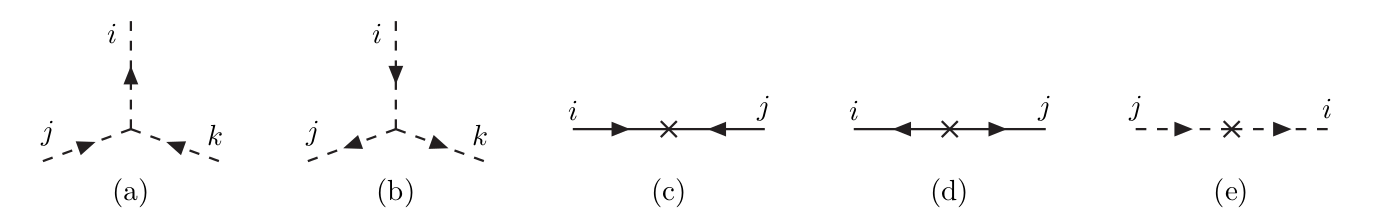
\includegraphics[scale=0.3]{feynman1.png}
            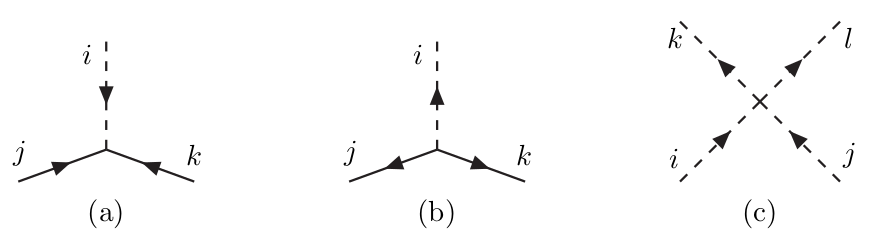
\includegraphics[scale=0.3]{feynman2.png}
        \end{figure}
\end{frame}

\begin{frame}
    
\end{frame}
    
\begin{frame}{Abelian gauge theories}
Let us introduce (abelian) gauge interactions. \\ 
Let us start with U(1) global symmetry 
\begin{equation*}
    \Phi_i \rightarrow e^{iq_i\Lambda_i}\Phi_i
\end{equation*}
The kinetic part of the lagrangian is always invariant
\begin{equation*}
    \mathcal{L}_{K} = \mathcal{L}_{WZ,D} = \int d^2\theta d^2 \bar\theta \Phi^*\Phi = \int d^2\theta -\frac{1}{4} \overline{D D} \Phi^*\Phi
\end{equation*}
The interaction part 
\begin{equation*}
    \mathcal{L}_{int} = \mathcal{L}_{WZ,F} = \int d^2\theta \frac{1}{2} \sum_{ij} \phi_i \phi_j + \frac{1}{3!} \sum_{ijk} \phi_i \phi_j \phi_k + \text{complex. conj.}
\end{equation*}
requires
\begin{equation*}
    m_{ij} = 0 \qquad \text{or} \qquad y_{ijk} = 0
\end{equation*}
whenever
\begin{equation*}
    q_i + q_j \neq 0 \qquad \text{or} \qquad q_i + q_j + q_k \neq 0
\end{equation*}
\end{frame}

\begin{frame}{Abelian gauge theories}
Promote to a local gauge symmetry
\begin{equation*}
    \Lambda \to \Lambda(x, \theta, \bar\theta)
\end{equation*}
\begin{itemize}
    \item Gauge parameter is now a supergauge field $\Lambda = \Lambda(x, \theta, \bar\theta)$
    \item Promote derivatives to covariant derivatives $\partial_\mu \to D_\mu = \partial_\mu + ieA_{\mu}$
    \item We need $\Lambda(x, \theta, \bar\theta)$ to be a left-chiral superfield if we want $\Phi'$ to be a left-chiral superfield (chain rule). \\ 
    \item Thus this causes a problem in the kinetic term because $\Lambda^*$ is a right-chiral superfield
    hence obviously $\Phi'^*\Phi' \neq \Phi^*\Phi$
    \item The problem is analogous to the kinetc term in "normal" when $\partial_u \phi^* \partial^\mu \phi$ was not gauge invariant
    \item Solution: add a term that compensate the gauge for the non invariant terms
\end{itemize}
\end{frame}

\begin{frame}{Abelian gauge theories}
\begin{equation*}
    \Phi^+\Phi \rightarrow \Phi^* e^{-i\Lambda^*(x)} e^{i\Lambda(x)} \Phi
\end{equation*}
$\Rightarrow$ need an object $A$ such that $A' = e^{i\Lambda*} A e^{-i\Lambda}$ and the 
quantity $\Phi^*A\Phi*$ is then gauge invariant. \\
Remember that a vector superfield $V$ transforms according to 
\begin{equation*}
    V \rightarrow V' = V + i{\Lambda* - \Lambda}
\end{equation*}
\centerline{$\Rightarrow \qquad A = e^V$ is what we need.} \\
Now we are just left with finding the gauge-invariant strength field term (euivalent of $F_{\mu\nu}F^{\mu\nu}$)
\end{frame}


\begin{frame}{Abelian gauge theories}
Let us start by defining the two chiral fields \\
\begin{equation*}
    \mathcal{W}_{\alpha}=-\frac{1}{4} \overline{D D} D_{\alpha} V, \quad \overline{\mathcal{W}}_{\dot{\alpha}} = -\frac{1}{4} D D \bar{D}_{\dot{\alpha}} V
\end{equation*}
where $V$ is a vector field. \\
The gauge-invariant dynamical term (equivalent to $F_{\mu\nu} F^{\mu\nu}$) is 
\begin{equation*}
   [W]_F + [\bar W]_F = \int d^2\theta W_{\alpha} W^{\alpha} + \int d^2\bar\theta \bar W_{\dot\alpha} \bar W^{\dot\alpha}
\end{equation*}
The explicit derivation is quite long (it will be put in the report appendix) but we can make two checks to get more convinced
\begin{itemize}
    \item Check that it is indeed gauge invariant
    \item Check that it contains the "normal" gauge strength field $F_{\mu\nu}F^{\mu\nu}$ after integrating out $\theta$ and $\bar\theta$
\end{itemize}
\end{frame}

\begin{frame}{Abelian gauge theories}
To see that it is gauge invariant:
\begin{equation*}
\begin{aligned}
    \mathcal{W}_{\alpha} \rightarrow-\frac{1}{4} \overline{D D} D_{\alpha}\left[V+i\left(\Omega^{*}-\Omega\right)\right] &=\mathcal{W}_{\alpha}+\frac{i}{4} \overline{D D} D_{\alpha} \Omega \\
    &=\mathcal{W}_{\alpha}-\frac{i}{4} \bar{D}^{\dot{\beta}}\left\{\bar{D}_{\dot{\beta}}, D_{\alpha}\right\} \Omega \\
    &=\mathcal{W}_{\alpha}+\frac{1}{2} \sigma_{\alpha \dot{\beta}}^{\mu} \partial_{\mu} \bar{D}^{\dot{\beta}} \Omega \\
    &=\mathcal{W}_{\alpha}
\end{aligned}
\end{equation*}
\end{frame}

\begin{frame}{Abelian gauge theories}
Remember that in the Wess-Zumino gauge the field expansion takes the form 
\begin{gather*}
    V(y, \theta, \bar \theta) = \bar\theta \bar{\sigma}^{\mu} \theta A_{\mu}(y)+\bar\theta \bar\theta \theta \lambda(y)+\theta \theta \bar\theta \lambda^{\dagger}(y) + \\ 
    \frac{1}{2} \theta \theta \theta \bar\theta \bar\theta\left[D(y)+i \theta_{\mu} A^{\mu}(y)\right]
\end{gather*}
Hence 
\begin{equation*}
    W = \dots
\end{equation*}
Finally 
\begin{equation*}
    \frac{1}{4}\left[\mathcal{WW}\right]_F + \frac{1}{4} \left[\overline{\mathcal{WW}}\right]_F = -\frac{1}{4} F_{\mu\nu} F^{\mu\nu} + i \lambda^{\dagger} \bar\sigma^{\mu} \partial_{\mu} \lambda + \frac{1}{2} D^2
\end{equation*}
We recovered the desired term $F_{\mu\nu}F^{\mu\nu}$, but what are the other two terms?
\end{frame}

\begin{frame}{Abelian gauge theories}
The term 
\begin{equation*}
    i\lambda^* \bar\sigma^{\mu}\partial_{\mu} \lambda
\end{equation*}
is just the superpartner of the photon, the \emph{photino}! \\
For the other term, we can show that it plays no physical role (as the F term in the chiral fields). To do this we need to spot all the $D$ dependence in our lagrangian. \\
Remembering that up to now our lagrangian is 
\begin{equation*}
    \mathcal{L} = \frac{1}{4}\left[\mathcal{WW}\right]_F + \frac{1}{4} \left[\overline{\mathcal{WW}}\right]_F + \left[\Phi^* e^V \Phi\right]_D + [W(\Phi)]_F + [\bar W(\Phi^*)]_F
\end{equation*}
once can note that the only other dependence on D is in $\left[\Phi^* e^V \Phi \right]_D = \Phi^*\Phi D$.
Hence the equation of motions for $D$ are
\begin{equation*}
    0 = \frac{\partial \mathcal{L}}{\partial D} = D + \Phi* \Phi 
\end{equation*}
\end{frame}

\begin{frame}{Abelian gauge theories}
Putting all together we get the SUSY QED lagrangian 
\begin{gather*}
    \mathcal{L} = \dots
\end{gather*}
To this we add another SUSY and supergauge invariant term $2[kV]_D = 2kD$ (e.o.m. is still algebraic). 
This term is called \emph{Fayet-Iliopoulos} and it will play an important role in the spontaneous SUSY breaking (next talks)
\begin{equation*}
    \boxed{\mathcal{L}_{SQED} = \dots}
\end{equation*}
\end{frame}

\begin{frame}{Non abelian gauge theories}
Now extend to generic gauge theories, in particular SU(n). In spacetime:
\begin{itemize}
    \item $n^2-1$ generators $T_{1}, \dots T_{n^2-1}$ (gauge fields)
    \item for $n=3$ we have 8 fields (gluons)
    \item $\left[T_a, T_b\right] = i \, f_{abc} \, T_c$ where $f_{abc}$ are called structure constants
    \item $U \in SU(n) \Rightarrow U = \exp(i g A^a T^a)$
    \item Covariant derivatives  in spacetime are $D_\mu = \partial_\mu - ig A_\mu = \partial_\mu - igA_u^a T^a$
\end{itemize}
In spacetime, guided by the fact that for $U(1)$ we had $$F_{\mu\nu} = \partial_\mu A_\nu - \partial_\nu A_\mu = \frac{i}{e} \, [D_\mu, D_\nu]$$
we \emph{define} our field strength tensor for a general gauge symmetry via 
\begin{equation*} 
    F_{\mu \nu} \equiv \frac{i}{g} \, [D_\mu, D_\nu] = \partial_\mu A_\nu - \partial_\nu A_\mu -ig \, [A_\mu, A_\nu]
\end{equation*}
$\Rightarrow$ how to extend to superspace?
\end{frame}

\begin{frame}{Non abelian gauge theories}
Our starting point is again a term like 
\begin{equation*}
    \Phi^* e^A \Phi
\end{equation*}
$\rightarrow$ we need to figure out how to set $A$
\end{frame}

\end{document}